\documentclass[a4paper,norsk, 10pt]{article}
\usepackage[utf8]{inputenc}
\usepackage{verbatim}
\usepackage{listings}
\usepackage{graphicx}
\usepackage[norsk]{babel}
\usepackage{a4wide}
\usepackage{color}
\usepackage{amsmath}
\usepackage{float}
\usepackage{amssymb}
\usepackage[dvips]{epsfig}
\usepackage[toc,page]{appendix}
\usepackage[T1]{fontenc}
\usepackage{cite} % [2,3,4] --> [2--4]
\usepackage{shadow}
\usepackage{hyperref}
\usepackage{titling}
\usepackage{marvosym }
\usepackage{subcaption}
\usepackage[noabbrev]{cleveref}
\usepackage{cite}


\setlength{\droptitle}{-10em}   % This is your set screw

\setcounter{tocdepth}{2}

\lstset{language=c++}
\lstset{alsolanguage=[90]Fortran}
\lstset{alsolanguage=Python}
\lstset{basicstyle=\small}
\lstset{backgroundcolor=\color{white}}
\lstset{frame=single}
\lstset{stringstyle=\ttfamily}
\lstset{keywordstyle=\color{red}\bfseries}
\lstset{commentstyle=\itshape\color{blue}}
\lstset{showspaces=false}
\lstset{showstringspaces=false}
\lstset{showtabs=false}
\lstset{breaklines}
\title{FYS2130 Oblig 3}
\author{Daniel Heinesen, daniehei}
\begin{document}
\maketitle

\section*{Diskusjon}

\subsection*{1)}
Eulers metode er av første orden(feil av orden $\Delta t$), og bruker bare ett punk til å tilnærme det neste punktet. Dette gjør at denne metoden er svært unøyaktig. Dette gjelder spesielt periodiske systemer, hvor Eulers metode ikke bevarer energi. Dette fører ofte til at man før enormt overdrevede resultater om man bruker denne metoden på slike systemer. \\

Runge Kutta 4(RK4) er en metode i Runge Kutta-familien. Denne familien bruker numerisk integralsjon til å løse differensiallikninger. RK4 bruker Simpsons regel for å løse disse integralene. RK4 bruke 4 punkter for å finne neste punkt. Dette betyr at den er veldig nøyaktig, og har en feil av orden $\Delta t^4$. Den bevarer også energi i periodiske systemer, noe som gjør den mye mer egnet til våre formål.

\section*{2)}


\section*{Regneoppgaver}

\section*{4)}
\subsection*{a)}
Verdiene som brukes i denne oppgaven er $m = 0.1$kg, $k = 10$N/m og $b = 0.1$kg/s. Med disse tallene vet vi at

$$
\gamma = \frac{b}{2m} = \frac{1}{2}, \qquad \omega = \sqrt{\frac{k}{m}} = 10
$$	

Dette betyr at

$$
\gamma < \omega
$$

Og vi har en underkritisk demping. Vi vet da at den analytiske løsningen er 

$$
z(t) = e^{-\gamma t}A\cos(\omega' t + \phi)
$$

hvor $\omega' = \sqrt{\omega^2 - \gamma^2} $, $A = x_0 = 0.1$m, og $\phi = 0$.\\

Koden finnes her \ref{lst:kode4a}(finnes også i filen \textit{pendulumRK4.py})\\

Jeg testet så programmet med 3 forskjellige tidssteg \textit{dt}, som er vist i figuren under

\begin{figure}[H]
    \centering
    \begin{subfigure}[b]{0.3\textwidth}
        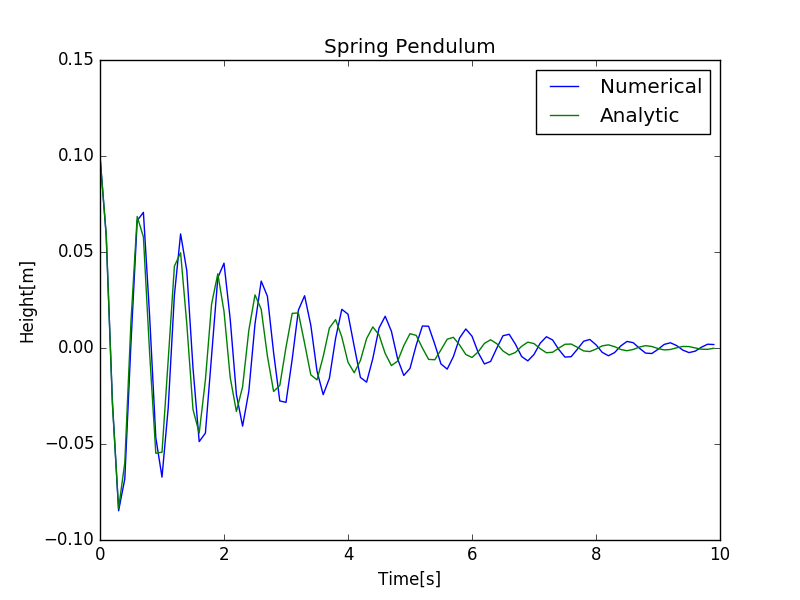
\includegraphics[width=\textwidth]{dt01.png}
        \caption{$dt = 0.1$}
        \label{fig:dt01}
    \end{subfigure}
    ~ %add desired spacing between images, e. g. ~, \quad, \qquad, \hfill etc. 
      %(or a blank line to force the subfigure onto a new line)
    \begin{subfigure}[b]{0.3\textwidth}
        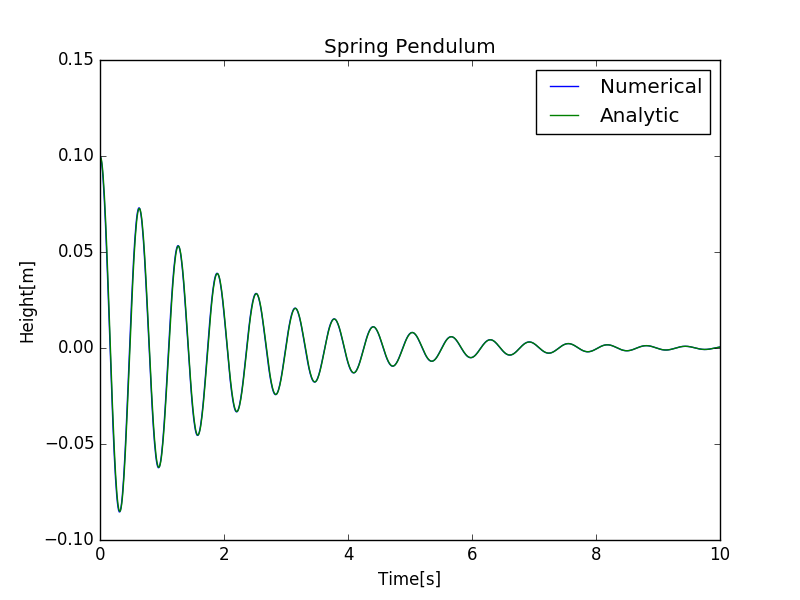
\includegraphics[width=\textwidth]{dt001.png}
        \caption{$dt = 0.01$}
        \label{fig:dt001}
    \end{subfigure}
    ~ %add desired spacing between images, e. g. ~, \quad, \qquad, \hfill etc. 
    %(or a blank line to force the subfigure onto a new line)
    \begin{subfigure}[b]{0.3\textwidth}
        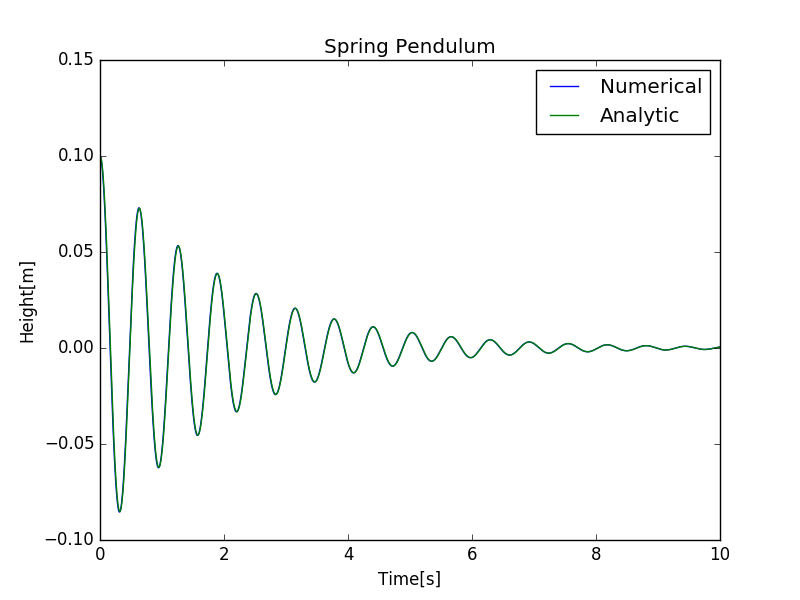
\includegraphics[width=\textwidth]{dt0001.png}
        \caption{$dt = 0.001$}
        \label{fig:dt001}
    \end{subfigure}
    \caption{Plot med 3 forskjellige tidssteg.}\label{fig:dter}
\end{figure}

Vi ser at $dt = 0.1$ er altfor smått og det er en klar forskjell mellom den numeriske og den analytiske løsningen. Forskjellen mellom $dt = 0.01$ og $0.001$ er derimot ikke så stor, og vi kan derfor si at den numerisk løsningen har stabilisert seg her. For å få den best mulige løsningen har jeg valgt å bruke $dt = 0.001$ videre.

\subsection*{b)}

Vi kan så se på hvordan systemet oppfører seg med overdemping, underdemping og ved kritisk demping. Jeg gjorde dette ved å justere verdiene for $b$

\begin{figure}[H]
\centering
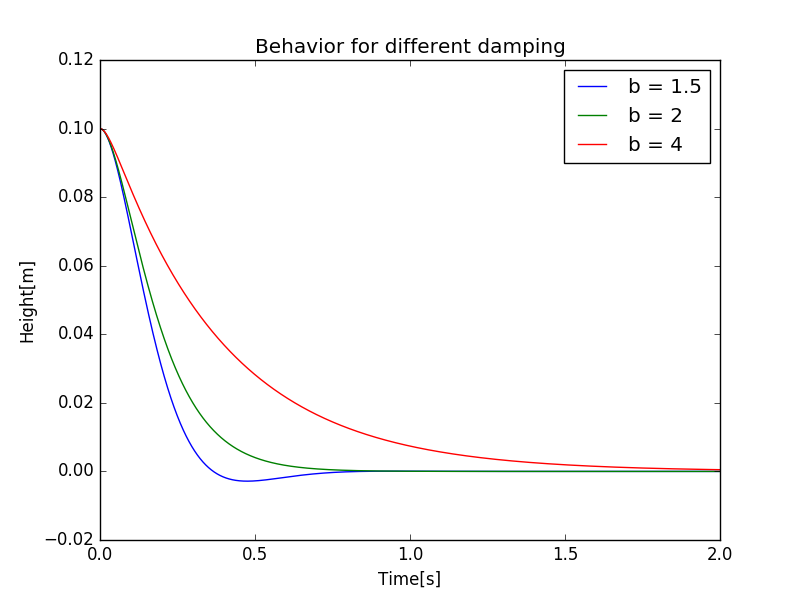
\includegraphics[scale=0.4]{diffdemp.png}
\caption{Figuren viser hvordan fjærpendelen oppfører seg for forskjellige verdier av dempingsfaktoren $b$}
\label{diffdemp}
\end{figure}

Verdiene til $b$ ble valgt ved å se på $\omega$ og $\gamma$. For å finne kritisk demping satt jeg 
$$
\omega = \gamma \Rightarrow b = 2m\sqrt{\frac{k}{m}} = 2
$$

For overkritisk demping ble må $b>2$ og for underkritiskdeming må $b<2$. Disse verdiene ble valg slik at plottene var lette å skille fra hverander.

\subsection*{c)}

Legger vi nå til en påtrykt kraft av formen

$$
F_0\cos(\omega_F t)
$$

Hvor $F_0 = 0.1$N. Forskjellige verdier av $\omega_F$ vil gi forskjellig oppførsel. Om $\omega_F = \omega$, vil systemet være i resonans, og ampituden vil øke til en $A_{max}$. Er dette ikke tilfelle vil størrelsen på amplituden variere periodisk. Her har jeg simulert begge tilfellene. Ca halvveis har jeg skrudd av den påtrykte kraften, slike at svigningene dempes og dør ut.

\begin{figure}[H]
\centering
\begin{subfigure}[b]{0.4\textwidth}
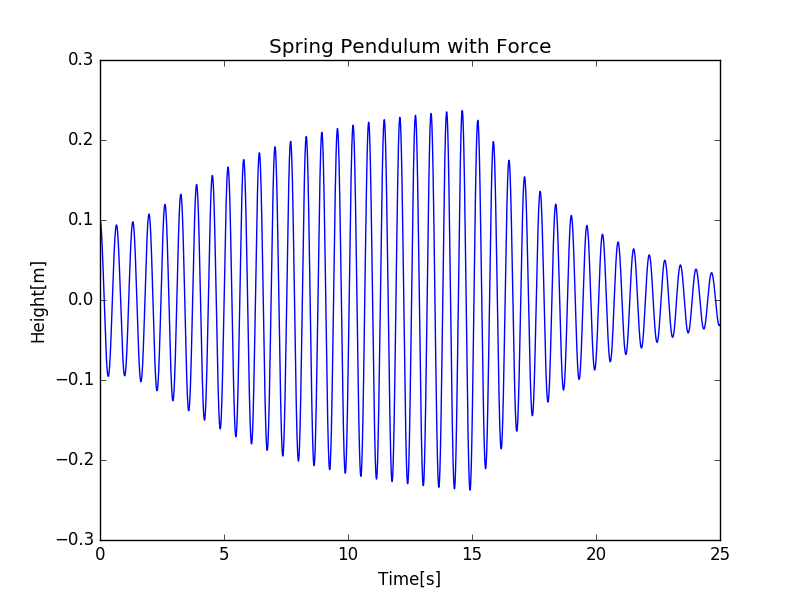
\includegraphics[width=\textwidth]{1omega.png}
\caption{$\omega_F = \omega$}
\end{subfigure}
~
\begin{subfigure}[b]{0.4\textwidth}
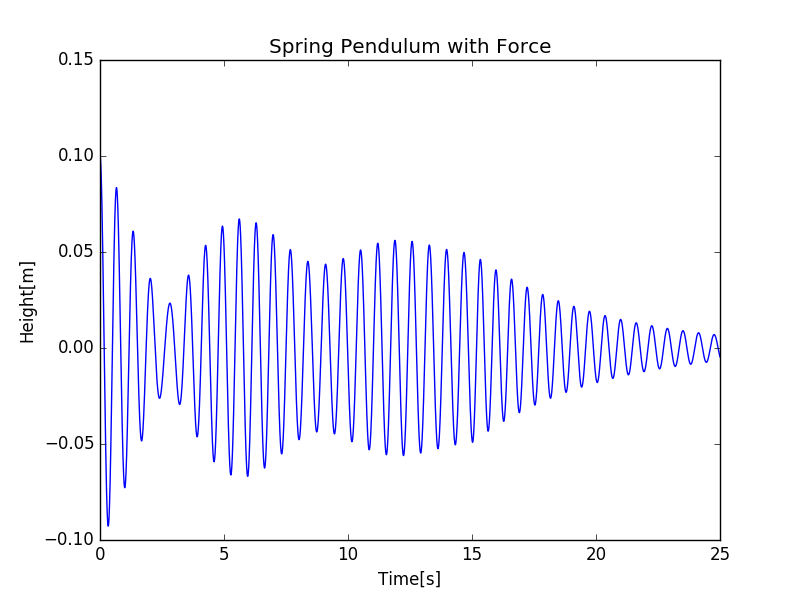
\includegraphics[width=\textwidth]{09omega.png}
\caption{$\omega_F = 0.9\omega$}
\end{subfigure}
\end{figure}

Vi kan se akkurat det vi forventet, om $\omega_F = \omega$ osillerer amplituden periodisk. Når kraften skrues av etter ca $15$ sek dør svigningene sakte ut.

\subsection*{d)}
Vi kan så sjekke hva frekvensresponsen til systemet er. Vi vil sjekke når svigningen har falt til $1/e$ av maksamplituden

\begin{figure}[H]
\centering
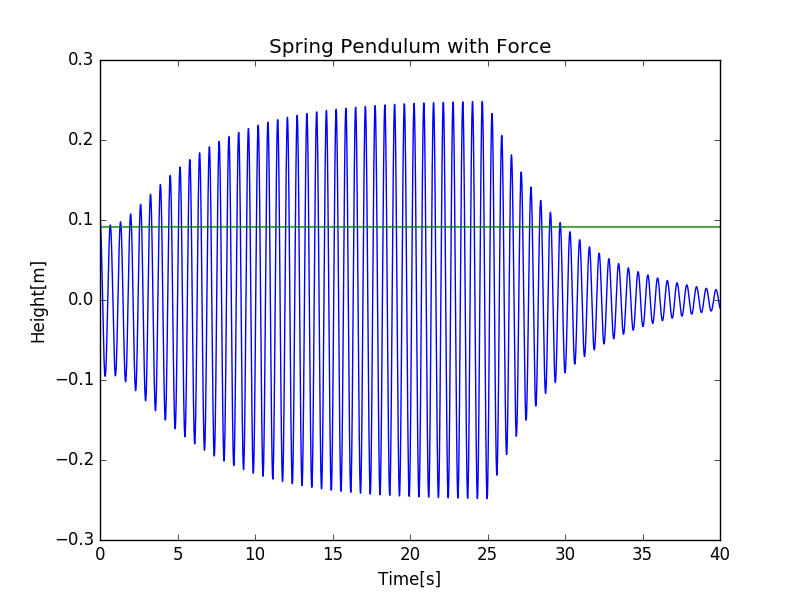
\includegraphics[scale=0.4]{oneOverEFall.png}
\caption{Den grønnelinjen viser hvor amplituden er $1/e$ av maksamplituden.}
\end{figure}

Er skrues den påtrykte kraften av etter $25$ sek. Vi kan se at amplituden krysser den grønne linjen ved ca $30$ sek. Med andre ord $\Delta t = 5$ sek. Vi kan nå finne Q-verdien

$$
Q = \omega \Delta t = \sqrt{\frac{b}{m}}\Delta t = \sqrt{\frac{0.04}{0.1}}5 = 3.16
$$

\section*{7)}



\section*{Kode:}

\subsection*{Kode for 4a)}


\lstinputlisting[caption = {Kode for 4a}, label = {lst:kode4a}]{pendulumRK4.py}

\end{document}